\documentclass[border=1mm]{standalone}

\usepackage[dvipsnames]{xcolor}
\usepackage{tikz}
\usetikzlibrary{positioning}

\usepackage[dvipsnames]{xcolor}
\usepackage{hyperref}

\colorlet{myblue}{RoyalBlue}
\colorlet{myred}{WildStrawberry}
\colorlet{myorange}{Melon}
\colorlet{mygreen}{OliveGreen}
\colorlet{myviolet}{RoyalPurple}
\colorlet{myyellow}{Goldenrod}
\hypersetup{urlbordercolor=Green, linkbordercolor=Blue}

\begin{document}
	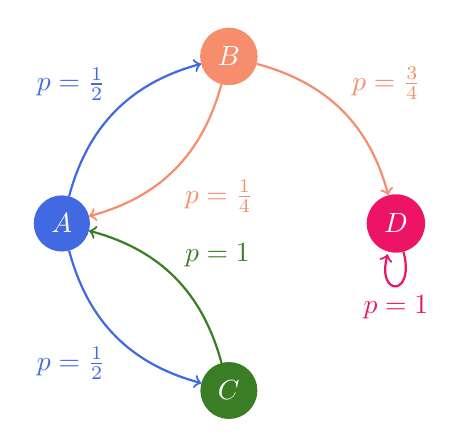
\begin{tikzpicture}[node distance={30mm}, thick, main/.style = {draw, circle, fill}]
		\node[main] (A) [color=myblue] {\textcolor{white}{$A$}};
		\node[main] (B) [above right of=A] [color=myorange] {\textcolor{white}{$B$}};
		\node[main] (C) [below right of=A] [color=mygreen] {\textcolor{white}{$C$}};
		\node[main] (D) [below right of=B] [color=myred] {\textcolor{white}{$D$}};
		\draw[->, thick, bend left=30, color=myblue] (A) edge node[midway, above left] {$p = \frac{1}{2}$} (B);
		\draw[->, thick, bend right=30, color=myblue] (A) edge node[midway, below left] {$p = \frac{1}{2}$} (C);
		
		\draw[->, thick, bend left=30, color=myorange] (B) edge node[midway, above right] {$p = \frac{3}{4}$} (D);
		\draw[->, thick, bend left=30, color=myorange] (B) edge node[midway, below right] {$p = \frac{1}{4}$} (A);
		
		\draw[->, thick, bend right=30, color=mygreen] (C) edge node[midway, above right] {$p = 1$} (A);
		
		\path[color=myred] (D) edge [anchor=center,loop below] node {$p = 1$} (D);
	\end{tikzpicture}
\end{document}